% Options for packages loaded elsewhere
\PassOptionsToPackage{unicode}{hyperref}
\PassOptionsToPackage{hyphens}{url}
%
\documentclass[
  a4paper,
]{book}
\usepackage{amsmath,amssymb}
\usepackage{iftex}
\ifPDFTeX
  \usepackage[T1]{fontenc}
  \usepackage[utf8]{inputenc}
  \usepackage{textcomp} % provide euro and other symbols
\else % if luatex or xetex
  \usepackage{unicode-math} % this also loads fontspec
  \defaultfontfeatures{Scale=MatchLowercase}
  \defaultfontfeatures[\rmfamily]{Ligatures=TeX,Scale=1}
\fi
\usepackage{lmodern}
\ifPDFTeX\else
  % xetex/luatex font selection
\fi
% Use upquote if available, for straight quotes in verbatim environments
\IfFileExists{upquote.sty}{\usepackage{upquote}}{}
\IfFileExists{microtype.sty}{% use microtype if available
  \usepackage[]{microtype}
  \UseMicrotypeSet[protrusion]{basicmath} % disable protrusion for tt fonts
}{}
\makeatletter
\@ifundefined{KOMAClassName}{% if non-KOMA class
  \IfFileExists{parskip.sty}{%
    \usepackage{parskip}
  }{% else
    \setlength{\parindent}{0pt}
    \setlength{\parskip}{6pt plus 2pt minus 1pt}}
}{% if KOMA class
  \KOMAoptions{parskip=half}}
\makeatother
\usepackage{xcolor}
\usepackage[top=3cm,left=3cm,right=2cm,bottom=2cm]{geometry}
\usepackage{longtable,booktabs,array}
\usepackage{calc} % for calculating minipage widths
% Correct order of tables after \paragraph or \subparagraph
\usepackage{etoolbox}
\makeatletter
\patchcmd\longtable{\par}{\if@noskipsec\mbox{}\fi\par}{}{}
\makeatother
% Allow footnotes in longtable head/foot
\IfFileExists{footnotehyper.sty}{\usepackage{footnotehyper}}{\usepackage{footnote}}
\makesavenoteenv{longtable}
\usepackage{graphicx}
\makeatletter
\def\maxwidth{\ifdim\Gin@nat@width>\linewidth\linewidth\else\Gin@nat@width\fi}
\def\maxheight{\ifdim\Gin@nat@height>\textheight\textheight\else\Gin@nat@height\fi}
\makeatother
% Scale images if necessary, so that they will not overflow the page
% margins by default, and it is still possible to overwrite the defaults
% using explicit options in \includegraphics[width, height, ...]{}
\setkeys{Gin}{width=\maxwidth,height=\maxheight,keepaspectratio}
% Set default figure placement to htbp
\makeatletter
\def\fps@figure{htbp}
\makeatother
\setlength{\emergencystretch}{3em} % prevent overfull lines
\providecommand{\tightlist}{%
  \setlength{\itemsep}{0pt}\setlength{\parskip}{0pt}}
\setcounter{secnumdepth}{5}
\usepackage{academicons}
\usepackage[portuguese]{babel}
\usepackage{booktabs}
\usepackage{draftwatermark}
\usepackage{fontspec}
\usepackage{fontawesome5}
\usepackage{float}
\usepackage{geometry}
\usepackage{graphicx}
\usepackage{letltxmacro}
\usepackage{longtable}
\usepackage[utf8]{inputenc}
\usepackage{pdfpages}
\usepackage[notransparent]{svg}
\usepackage{tcolorbox}
\usepackage{titlesec}
\usepackage{tocloft}
\usepackage{url}
\usepackage{xcolor}
\usepackage[linktoc=all]{hyperref}

\SetWatermarkLightness{0.9}
\SetWatermarkText{RASCUNHO}
\SetWatermarkScale{1}

\AtBeginDocument{\let\maketitle\relax}

\renewcommand{\href}[2]{#2\footnote{\url{#1}}}

\definecolor{lightgray}{gray}{0.95}

\newtcolorbox{blackbox}{
  colback=lightgray,
  colframe=orange,
  coltext=black,
  boxsep=5pt,
  arc=4pt}
\newenvironment{infobox}[1]
  {
  \begin{itemize}
  \renewcommand{\labelitemi}{
    \raisebox{-.7\height}[0pt][0pt]{
      {\setkeys{Gin}{width=3em,keepaspectratio}
        \includegraphics{#1}}
    }
  }
  \setlength{\fboxsep}{1em}
  \begin{blackbox}
  \item
  }
  {
  \end{blackbox}
  \end{itemize}
  }


\LetLtxMacro\Oldfootnote\footnote
\newcommand{\EnableFootNotes}{%
  \LetLtxMacro\footnote\Oldfootnote%
}
\newcommand{\DisableFootNotes}{%
  \renewcommand{\footnote}[2][]{\relax}
}
\ifLuaTeX
  \usepackage{selnolig}  % disable illegal ligatures
\fi
\IfFileExists{bookmark.sty}{\usepackage{bookmark}}{\usepackage{hyperref}}
\IfFileExists{xurl.sty}{\usepackage{xurl}}{} % add URL line breaks if available
\urlstyle{same}
\hypersetup{
  pdftitle={Autoavaliação},
  hidelinks,
  pdfcreator={LaTeX via pandoc}}

\title{Autoavaliação}
\author{}
\date{\vspace{-2.5em}}

\begin{document}
\maketitle

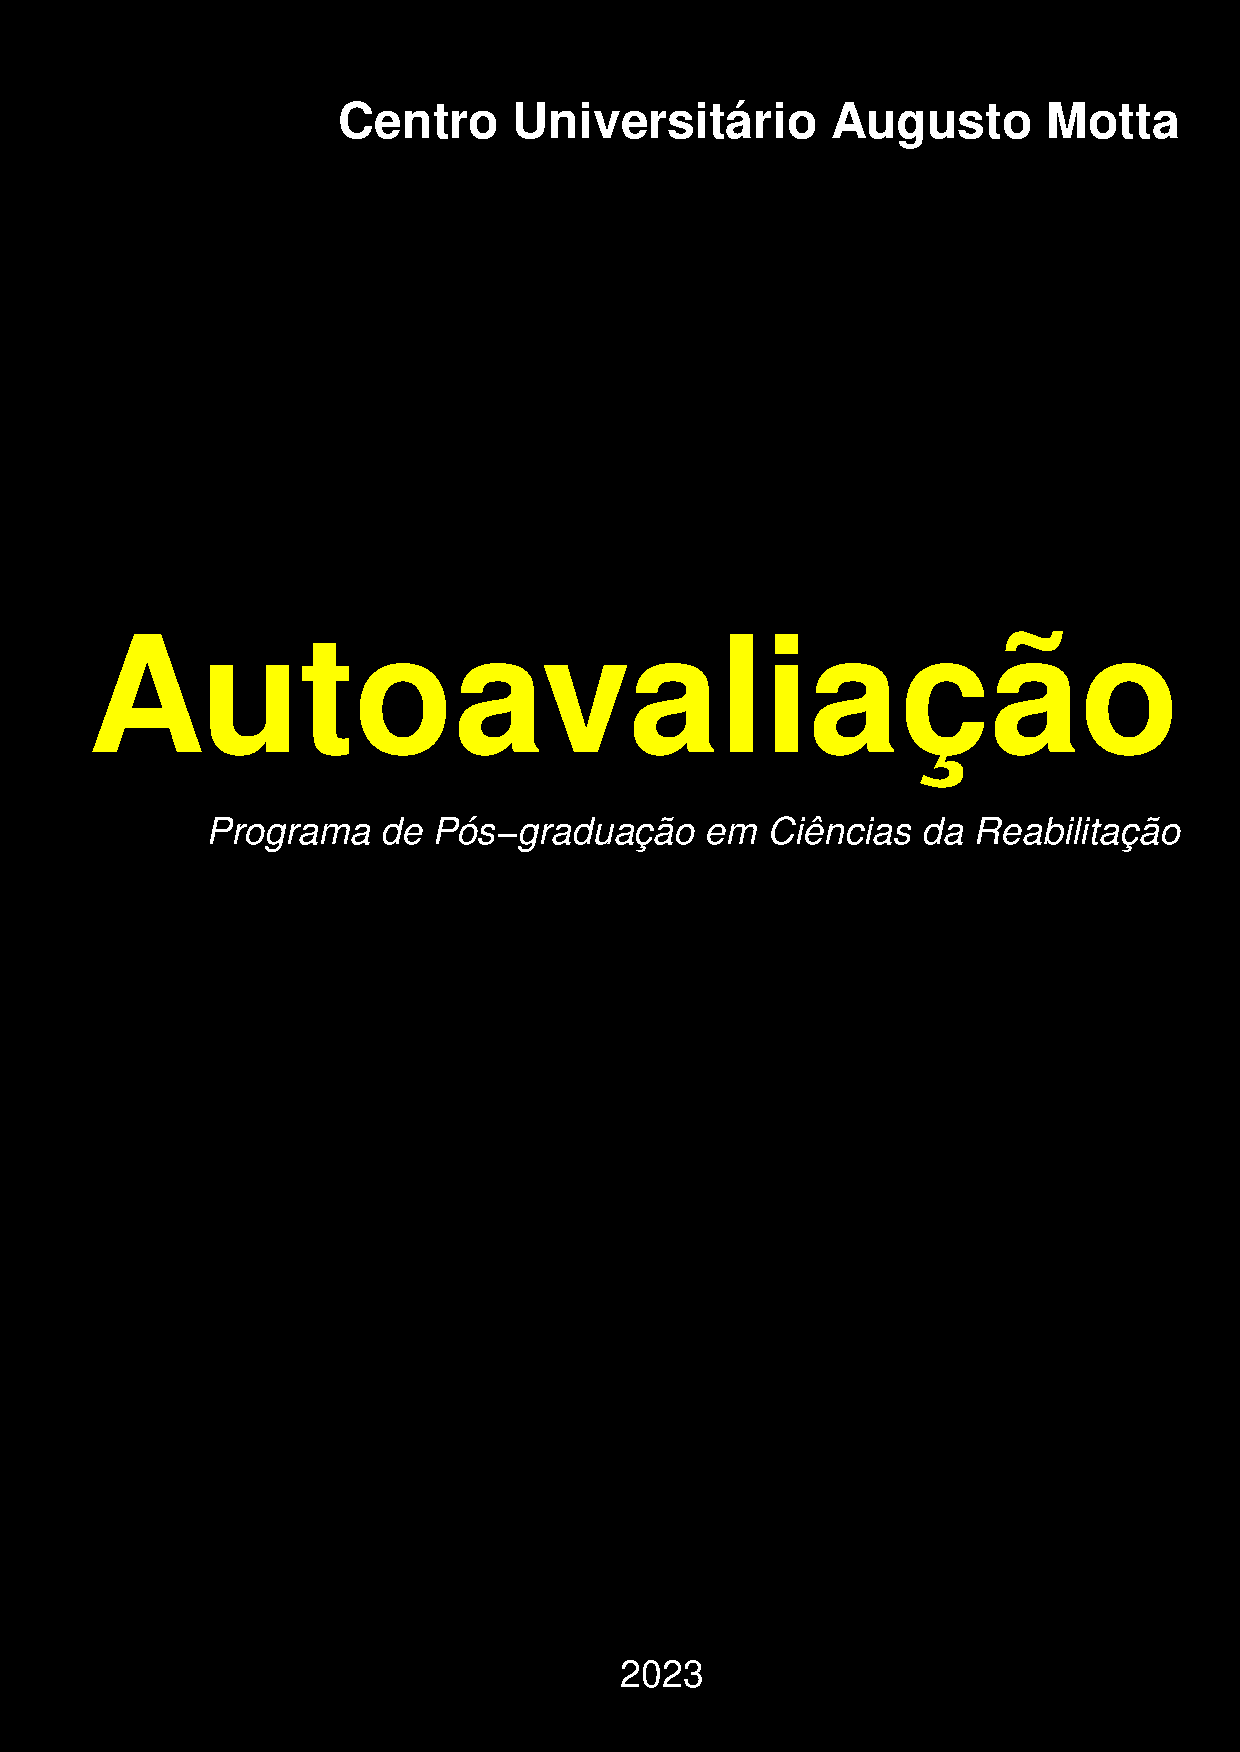
\includepdf[pages={1},noautoscale=false, fitpaper=true, width=8.27in, height=11.69in, frame=false, trim=0mm 0mm 0mm 0mm, clip, offset=0mm 0mm]{covers/Cover_1.pdf}
\newpage

{
\setcounter{tocdepth}{1}
\tableofcontents
}
\mainmatter
\clearpage
\markboth{}{}

\mainmatter
\clearpage
\markboth{}{}

\href{https://twitter.com/share?url=}{} \href{https://www.facebook.com/sharer.php?u=}{} \href{https://www.linkedin.com/shareArticle?mini=true\&url=}{}

\hypertarget{metodologia}{%
\section*{\texorpdfstring{\textbf{Metodologia}}{Metodologia}}\label{metodologia}}
\addcontentsline{toc}{section}{\textbf{Metodologia}}

\newpage

\hypertarget{resultados}{%
\section*{\texorpdfstring{\textbf{Resultados}}{Resultados}}\label{resultados}}
\addcontentsline{toc}{section}{\textbf{Resultados}}

\hypertarget{suxedntese-dos-dados}{%
\subsection*{\texorpdfstring{\textbf{Síntese dos dados}}{Síntese dos dados}}\label{suxedntese-dos-dados}}
\addcontentsline{toc}{subsection}{\textbf{Síntese dos dados}}

\hypertarget{dados-completos--}{%
\subsubsection{\texorpdfstring{\textbf{Dados completos \{-\}}}{Dados completos \{-\}}}\label{dados-completos--}}

\hypertarget{dados-perdidos--}{%
\subsubsection{\texorpdfstring{\textbf{Dados perdidos \{-\}}}{Dados perdidos \{-\}}}\label{dados-perdidos--}}

\hypertarget{documentos-capes}{%
\subsection*{\texorpdfstring{\textbf{Documentos CAPES}}{Documentos CAPES}}\label{documentos-capes}}
\addcontentsline{toc}{subsection}{\textbf{Documentos CAPES}}

\newpage

\hypertarget{programa}{%
\section{\texorpdfstring{\textbf{1. Programa}}{1. Programa}}\label{programa}}

\hypertarget{section}{%
\subsection{\texorpdfstring{\textbf{1.1.1}}{1.1.1}}\label{section}}

\hypertarget{estrutura-acaduxeamica-do-programa}{%
\subsubsection{\texorpdfstring{\textbf{Estrutura Acadêmica do Programa}}{Estrutura Acadêmica do Programa}}\label{estrutura-acaduxeamica-do-programa}}

\hypertarget{objetivos}{%
\paragraph{\texorpdfstring{\textbf{Objetivos}}{Objetivos}}\label{objetivos}}

\hypertarget{perfil-do-egresso}{%
\paragraph{\texorpdfstring{\textbf{Perfil do egresso}}{Perfil do egresso}}\label{perfil-do-egresso}}

\hypertarget{descricao-ac}{%
\paragraph{\texorpdfstring{\textbf{AC}}{AC}}\label{descricao-ac}}

\hypertarget{descricao-lp}{%
\paragraph{\texorpdfstring{\textbf{LP}}{LP}}\label{descricao-lp}}

\hypertarget{descricao-pp}{%
\paragraph{\texorpdfstring{\textbf{PP}}{PP}}\label{descricao-pp}}

\hypertarget{docentes-linhas-pesquisa}{%
\paragraph{\texorpdfstring{\textbf{Docentes}}{Docentes}}\label{docentes-linhas-pesquisa}}

\hypertarget{posdocs-linhas-pesquisa}{%
\paragraph{\texorpdfstring{\textbf{Pós-Docs}}{Pós-Docs}}\label{posdocs-linhas-pesquisa}}

\hypertarget{coerencia-quantitativo}{%
\paragraph{\texorpdfstring{\textbf{Síntese}}{Síntese}}\label{coerencia-quantitativo}}

Área de Concentração \textbar{} Dados individuais

Linhas de pesquisa \textbar{} Dados individuais

Projetos de pesquisa \textbar{} Dados individuais

Docentes \textbar{} Dados individuais

Pós-Docs \textbar{} Dados individuais

\hypertarget{section-1}{%
\subsection{\texorpdfstring{\textbf{1.1.2}}{1.1.2}}\label{section-1}}

\hypertarget{proposta-curricular-do-programa}{%
\subsubsection{\texorpdfstring{\textbf{Proposta Curricular do Programa}}{Proposta Curricular do Programa}}\label{proposta-curricular-do-programa}}

\hypertarget{qualitativa}{%
\paragraph{\texorpdfstring{\emph{Qualitativa}}{Qualitativa}}\label{qualitativa}}

\emph{Em construção}

Início ~⬆️

\hypertarget{quantitativa}{%
\paragraph{\texorpdfstring{\emph{Quantitativa}}{Quantitativa}}\label{quantitativa}}

\hypertarget{section-2}{%
\subsection{\texorpdfstring{\textbf{1.1.3}}{1.1.3}}\label{section-2}}

\hypertarget{infraestrutura}{%
\subsubsection{\texorpdfstring{\textbf{Infraestrutura}}{Infraestrutura}}\label{infraestrutura}}

\emph{Em construção}

Início ~⬆️

\hypertarget{section-3}{%
\subsection{\texorpdfstring{\textbf{1.2.1}}{1.2.1}}\label{section-3}}

\hypertarget{dimensuxe3o-do-corpo-docente-permanente}{%
\subsubsection{\texorpdfstring{\textbf{Dimensão do corpo Docente Permanente}}{Dimensão do corpo Docente Permanente}}\label{dimensuxe3o-do-corpo-docente-permanente}}

Dimensão \textbar{} Dados individuais

Vínculo \textbar{} Dados individuais

Regime de trabalho \textbar{} Dados individuais

Carga horária PG \textbar{} Dados individuais

\hypertarget{section-4}{%
\subsection{\texorpdfstring{\textbf{1.2.2}}{1.2.2}}\label{section-4}}

\hypertarget{coeruxeancia-acaduxeamica-do-corpo-docente-uxe0-proposta-do-ppg}{%
\subsubsection{\texorpdfstring{\textbf{Coerência acadêmica do Corpo Docente à proposta do PPG}}{Coerência acadêmica do Corpo Docente à proposta do PPG}}\label{coeruxeancia-acaduxeamica-do-corpo-docente-uxe0-proposta-do-ppg}}

Área de conhecimento titulação \textbar{} Dados individuais

\hypertarget{section-5}{%
\subsection{\texorpdfstring{\textbf{1.2.3}}{1.2.3}}\label{section-5}}

\hypertarget{estabilidade-do-corpo-docente-permanente}{%
\subsubsection{\texorpdfstring{\textbf{Estabilidade do corpo docente permanente}}{Estabilidade do corpo docente permanente}}\label{estabilidade-do-corpo-docente-permanente}}

\emph{Em construção}

Início ~⬆️

\hypertarget{section-6}{%
\subsection{\texorpdfstring{\textbf{1.2.4}}{1.2.4}}\label{section-6}}

\hypertarget{percentual-de-docentes-permanentes-com-dedicauxe7uxe3o-exclusiva-ao-ppg}{%
\subsubsection{\texorpdfstring{\textbf{Percentual de docentes permanentes com dedicação exclusiva ao PPG}}{Percentual de docentes permanentes com dedicação exclusiva ao PPG}}\label{percentual-de-docentes-permanentes-com-dedicauxe7uxe3o-exclusiva-ao-ppg}}

\emph{Em construção}

Início ~⬆️

\hypertarget{section-7}{%
\subsection{\texorpdfstring{\textbf{1.2.5}}{1.2.5}}\label{section-7}}

\hypertarget{capacidade-de-captauxe7uxe3o-de-recursos}{%
\subsubsection{\texorpdfstring{\textbf{Capacidade de captação de recursos}}{Capacidade de captação de recursos}}\label{capacidade-de-captauxe7uxe3o-de-recursos}}

\hypertarget{section-8}{%
\subsection{\texorpdfstring{\textbf{1.3.1}}{1.3.1}}\label{section-8}}

\hypertarget{adequauxe7uxe3o-da-proposta-ao-plano-institucional-da-ies}{%
\subsubsection{\texorpdfstring{\textbf{Adequação da proposta ao Plano Institucional da IES}}{Adequação da proposta ao Plano Institucional da IES}}\label{adequauxe7uxe3o-da-proposta-ao-plano-institucional-da-ies}}

\hypertarget{section-9}{%
\subsection{\texorpdfstring{\textbf{1.3.2}}{1.3.2}}\label{section-9}}

\hypertarget{adequauxe7uxe3o-do-planejamento}{%
\subsubsection{\texorpdfstring{\textbf{Adequação do planejamento}}{Adequação do planejamento}}\label{adequauxe7uxe3o-do-planejamento}}

\emph{Em construção}

Início ~⬆️

\hypertarget{section-10}{%
\subsection{\texorpdfstring{\textbf{1.4.1}}{1.4.1}}\label{section-10}}

\hypertarget{adequauxe7uxe3o-dos-processos-e-procedimentos-utilizados-para-a-autoavaliauxe7uxe3o-do-programa}{%
\subsubsection{\texorpdfstring{\textbf{Adequação dos processos e procedimentos utilizados para a autoavaliação do Programa}}{Adequação dos processos e procedimentos utilizados para a autoavaliação do Programa}}\label{adequauxe7uxe3o-dos-processos-e-procedimentos-utilizados-para-a-autoavaliauxe7uxe3o-do-programa}}

\emph{Em construção}

Início ~⬆️

\newpage

\hypertarget{formacao}{%
\section{\texorpdfstring{\textbf{2. Formação}}{2. Formação}}\label{formacao}}

\hypertarget{section-11}{%
\subsection{\texorpdfstring{\textbf{2.1.1}}{2.1.1}}\label{section-11}}

\hypertarget{coeruxeancia-do-produto-final}{%
\subsubsection{\texorpdfstring{\textbf{Coerência do produto final}}{Coerência do produto final}}\label{coeruxeancia-do-produto-final}}

\emph{Em construção}

Início ~⬆️

\hypertarget{section-12}{%
\subsection{\texorpdfstring{\textbf{2.1.2}}{2.1.2}}\label{section-12}}

\hypertarget{qualidade-do-produto-final}{%
\subsubsection{\texorpdfstring{\textbf{Qualidade do produto final}}{Qualidade do produto final}}\label{qualidade-do-produto-final}}

\emph{Em construção}

Início ~⬆️

\hypertarget{section-13}{%
\subsection{\texorpdfstring{\textbf{2.2.1}}{2.2.1}}\label{section-13}}

\hypertarget{produuxe7uxe3o-do-corpo-discente-em-eventos-cientuxedficos}{%
\subsubsection{\texorpdfstring{\textbf{Produção do corpo discente em eventos científicos}}{Produção do corpo discente em eventos científicos}}\label{produuxe7uxe3o-do-corpo-discente-em-eventos-cientuxedficos}}

\emph{Em construção}

Início ~⬆️

\hypertarget{section-14}{%
\subsection{\texorpdfstring{\textbf{2.2.2}}{2.2.2}}\label{section-14}}

\hypertarget{produuxe7uxe3o-bibliogruxe1fica-dos-discentesegressos-acaduxeamico}{%
\subsubsection{\texorpdfstring{\textbf{Produção bibliográfica dos discentes/egressos -- Acadêmico}}{Produção bibliográfica dos discentes/egressos -- Acadêmico}}\label{produuxe7uxe3o-bibliogruxe1fica-dos-discentesegressos-acaduxeamico}}

\emph{Em construção}

Início ~⬆️

\hypertarget{section-15}{%
\subsection{\texorpdfstring{\textbf{2.3.1}}{2.3.1}}\label{section-15}}

\hypertarget{atuauxe7uxe3o-dos-egressos}{%
\subsubsection{\texorpdfstring{\textbf{Atuação dos Egressos}}{Atuação dos Egressos}}\label{atuauxe7uxe3o-dos-egressos}}

\emph{Em construção}

Início ~⬆️

\hypertarget{section-16}{%
\subsection{\texorpdfstring{\textbf{2.3.2}}{2.3.2}}\label{section-16}}

\hypertarget{egressos-de-destaque-na-sociedade}{%
\subsubsection{\texorpdfstring{\textbf{Egressos de destaque na sociedade}}{Egressos de destaque na sociedade}}\label{egressos-de-destaque-na-sociedade}}

\emph{Em construção}

Início ~⬆️

\hypertarget{section-17}{%
\subsection{\texorpdfstring{\textbf{2.4.1}}{2.4.1}}\label{section-17}}

\hypertarget{produuxe7uxe3o-bibliogruxe1fica-total-do-programa-acaduxeamico}{%
\subsubsection{\texorpdfstring{\textbf{Produção bibliográfica total do Programa -- Acadêmico}}{Produção bibliográfica total do Programa -- Acadêmico}}\label{produuxe7uxe3o-bibliogruxe1fica-total-do-programa-acaduxeamico}}

\emph{Em construção}

Início ~⬆️

\hypertarget{section-18}{%
\subsection{\texorpdfstring{\textbf{2.5.1}}{2.5.1}}\label{section-18}}

\hypertarget{atividades-de-ensino-nas-disciplinas-do-ppg}{%
\subsubsection{\texorpdfstring{\textbf{Atividades de ensino nas disciplinas do PPG}}{Atividades de ensino nas disciplinas do PPG}}\label{atividades-de-ensino-nas-disciplinas-do-ppg}}

\hypertarget{section-19}{%
\subsection{\texorpdfstring{\textbf{2.5.2}}{2.5.2}}\label{section-19}}

\hypertarget{responsabilidade-por-ppptt}{%
\subsubsection{\texorpdfstring{\textbf{Responsabilidade por PP/PTT}}{Responsabilidade por PP/PTT}}\label{responsabilidade-por-ppptt}}

\emph{Em construção}

Início ~⬆️

\hypertarget{section-20}{%
\subsection{\texorpdfstring{\textbf{2.5.3}}{2.5.3}}\label{section-20}}

\hypertarget{orientauxe7uxe3o-no-ppg}{%
\subsubsection{\texorpdfstring{\textbf{Orientação no PPG}}{Orientação no PPG}}\label{orientauxe7uxe3o-no-ppg}}

\emph{Em construção}

Início ~⬆️

\hypertarget{section-21}{%
\subsection{\texorpdfstring{\textbf{2.5.4}}{2.5.4}}\label{section-21}}

\hypertarget{titulauxe7uxe3o-no-ppg}{%
\subsubsection{\texorpdfstring{\textbf{Titulação no PPG}}{Titulação no PPG}}\label{titulauxe7uxe3o-no-ppg}}

\emph{Em construção}

Início ~⬆️

\hypertarget{section-22}{%
\subsection{\texorpdfstring{\textbf{2.5.5}}{2.5.5}}\label{section-22}}

\hypertarget{orientauxe7uxe3o-na-graduauxe7uxe3o}{%
\subsubsection{\texorpdfstring{\textbf{Orientação na graduação}}{Orientação na graduação}}\label{orientauxe7uxe3o-na-graduauxe7uxe3o}}

\emph{Em construção}

Início ~⬆️

\newpage

\hypertarget{impacto}{%
\section{\texorpdfstring{\textbf{3. Impacto na sociedade}}{3. Impacto na sociedade}}\label{impacto}}

\hypertarget{section-23}{%
\subsection{\texorpdfstring{\textbf{3.1.1}}{3.1.1}}\label{section-23}}

\hypertarget{produuxe7uxe3o-bibliogruxe1fica-indicada-dos-dp-acaduxeamico}{%
\subsubsection{\texorpdfstring{\textbf{Produção bibliográfica indicada dos DP -- Acadêmico}}{Produção bibliográfica indicada dos DP -- Acadêmico}}\label{produuxe7uxe3o-bibliogruxe1fica-indicada-dos-dp-acaduxeamico}}

\emph{Em construção}

Início ~⬆️

\hypertarget{section-24}{%
\subsection{\texorpdfstring{\textbf{3.1.2}}{3.1.2}}\label{section-24}}

\hypertarget{produuxe7uxe3o-do-programa}{%
\subsubsection{\texorpdfstring{\textbf{Produção do Programa}}{Produção do Programa}}\label{produuxe7uxe3o-do-programa}}

Produção por Área de Concentração \textbar{} Dados individuais

Produção por Linha de Pesquisa \textbar{} Dados individuais

Produção por tipo \textbar{} Dados individuais

Categoria do Autor Principal \textbar{} Dados individuais

Produção vinculada à TCC \textbar{} Dados individuais

Produção bibliográfica \textbar{} Dados individuais

Produção técnica \textbar{} Dados individuais

\hypertarget{section-25}{%
\subsection{\texorpdfstring{\textbf{3.2.1}}{3.2.1}}\label{section-25}}

\hypertarget{avaliauxe7uxe3o-quantitativa-dos-impactos-do-ppg}{%
\subsubsection{\texorpdfstring{\textbf{Avaliação quantitativa dos impactos do PPG}}{Avaliação quantitativa dos impactos do PPG}}\label{avaliauxe7uxe3o-quantitativa-dos-impactos-do-ppg}}

\emph{Em construção}

Início ~⬆️

\hypertarget{section-26}{%
\subsection{\texorpdfstring{\textbf{3.2.2}}{3.2.2}}\label{section-26}}

\hypertarget{avaliauxe7uxe3o-qualitativa-dos-impactos-do-ppg}{%
\subsubsection{\texorpdfstring{\textbf{Avaliação qualitativa dos impactos do PPG}}{Avaliação qualitativa dos impactos do PPG}}\label{avaliauxe7uxe3o-qualitativa-dos-impactos-do-ppg}}

\emph{Em construção}

Início ~⬆️

\hypertarget{section-27}{%
\subsection{\texorpdfstring{\textbf{3.3.1}}{3.3.1}}\label{section-27}}

\hypertarget{visibilidade}{%
\subsubsection{\texorpdfstring{\textbf{Visibilidade}}{Visibilidade}}\label{visibilidade}}

\emph{Em construção}

Início ~⬆️

\hypertarget{section-28}{%
\subsection{\texorpdfstring{\textbf{3.3.2}}{3.3.2}}\label{section-28}}

\hypertarget{internacionalizauxe7uxe3o-e-inseruxe7uxe3o}{%
\subsubsection{\texorpdfstring{\textbf{Internacionalização e Inserção}}{Internacionalização e Inserção}}\label{internacionalizauxe7uxe3o-e-inseruxe7uxe3o}}

\emph{Em construção}

Início ~⬆️

\end{document}
